This chapter discusses the redundancy and scalability of the proposed load balancers.
The ECMP technique is expected to make the load balancers redundant and scalable since all the load balancer containers act as active.
The whole system is resilient to a single failure of load balancer container.
Also since multiple of load balancers can be utilized simultaneously, it is expected that the throughput of the total system is increased significantly.
In order to evaluate these characteristics of the ECMP technique,
the author examined if the ECMP routing table is updated correctly when multiple of the load balancer {\em pods} are started.
After that, in order to explore the scalability, the author also measured the throughput of the cluster of load balancers.
Finally, the author examined how quick those ECMP routing table updates are.
The following subsections explain the evaluation in detail.

\section{Evaluation method}

\begin{figure}[b]
  \centering
    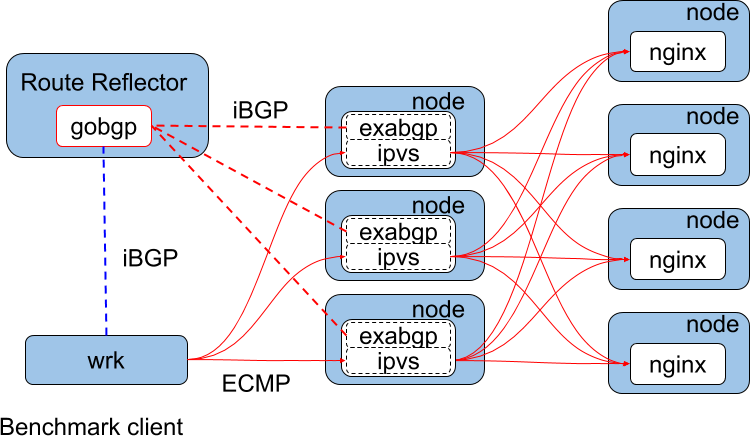
\includegraphics[width=0.9\columnwidth]{Figs/lb_ecmp_schem}
    \caption{Experimental setups.}
    \label{fig:lb_ecmp_schem}
\end{figure}

\begin{table}[b]
  \centering
  \begin{tabular}{ll}
    \hline \\
    \multicolumn{2}{l}{[Hardware Specification]}   \\
    & CPU: Xeon E5-2450 2.10GHz x 8 (with Hyper Threading) \\
    & Memory: 32GB \\
    & NIC: Broadcom BCM5720 Giga bit \\
    & (Node x 6, Load Balancer x 4) \\
    & \\
    & CPU: Xeon E5-2450 2.10GHz x 8 (with Hyper Threading) \\
    & Memory: 32GB \\
    & NIC: Intel X550 \\
    & (Client x 1) \\
    & \\
    \multicolumn{2}{l}{[Node Software]}  \\
    & OS: Debian 9.5, linux-4.16.8 \\
    & Kubernetes v1.5.2 \\
    & flannel v0.7.0 \\
    & etcd version: 3.0.15 \\
    & \\
    \multicolumn{2}{l}{[Container Software]}   \\
    & Keepalived: v1.3.2 (12/03,2016) \\
    & nginx : 1.15.4(web server) \\
    \\ \hline
  \end{tabular}
  \caption{Hardware and software specifications.}
  \label{tab:ecmp-hw_sw_spec}
\end{table}

Figure~\ref{fig:lb_ecmp_schem} shows the schematic diagram of the experimental setup and Table~\ref{tab:ecmp-hw_sw_spec} summarizes hardware and software specifications for the experiments.

Multiple {\em pods} are deployed on multiple nodes in the Kubernetes cluster.
In each {\em pod}, an nginx web server pod that returns the IP address of the {\em pod} are running.
There are multiple nodes for load balancers and on each of the nodes, single load balancer {\em pod} is deployed.
Each load balancer {\em pod} consists of both an ipvs container and an exabgp container.
The routing table of the benchmark client is updated by BGP protocol through a route reflector.

Using these hardware and software setups, the following four types of evaluations have been carried out;
1) Evaluation of ECMP functionality. The author examined if ECMP routing table is correctly updated.
3) Evaluation of the scalability. The author evaluated how throughput is improved by running multiple ipvs pods.
2) Evaluation of ECMP response. The author evaluated the delay between the time ipvs pods are started or stopped until the time ECMP routing table reflected the change.

The throughputs are measured using wrk in the same manner as in Chapter~\ref{chapter:portablelb}.
Notable differences from the previous throughput experiment in Figure~\ref{fig:benchmark-setup} are;
There four nodes for load balancers instead of one.
And the 10 Gbps NIC is used for the benchmark client since for scalability experiment we have multiple of ipvs container load balancers that can fill up 1 Gbps bandwidth.
Some of the software has also been updated to the most recent versions at the time of the experiment.

\FloatBarrier

\section{ECMP functionality}

\begin{table}[h]

  \begin{subtable}{.9\textwidth}
  \centering
  \begin{tabular}{l}
    \hline 
    10.1.1.0/24 via 10.0.0.106 dev eth0 proto zebra metric 20 \\
    \hline
  \end{tabular}
  \caption{With single load balancer {\em pod}.}
  \label{tab:single}
\end{subtable}

\begin{subtable}{.9\textwidth}
  \centering
  \begin{tabular}{ll}
    \hline
    \multicolumn{2}{l}{10.1.1.0/24 proto zebra metric 20 } \\
    \hspace{15 mm}
    & nexthop via 10.0.0.105  dev eth0 weight 1 \\
    & nexthop via 10.0.0.106  dev eth0 weight 1 \\
    & nexthop via 10.0.0.107  dev eth0 weight 1 \\
    \hline
  \end{tabular}
  \caption{With three load balancer {\em pod}s.}
  \label{tab:three}
\end{subtable}

\begin{subtable}{.9\textwidth}
  \centering
  \begin{tabular}{ll}
    \hline
    \multicolumn{2}{l}{10.1.1.0/24 pro to zebra metric 20 } \\
    \hspace{15 mm}
    & nexthop via 10.0.0.107  dev eth0 weight 1 \\
    & nexthop via 10.0.0.105  dev eth0 weight 1 \\
    & nexthop via 10.0.0.106  dev eth0 weight 1 \\
    \multicolumn{2}{l}{10.1.2.0/24 proto zebra metric 20 } \\
    \hspace{15 mm}
    & nexthop via 10.0.0.107  dev eth0 weight 1 \\
    & nexthop via 10.0.0.106  dev eth0 weight 1 \\
    \hline
  \end{tabular}
  \caption{For a service with three load balancer {\em pod}s and a service with two load balancer {\em pod}s.}
  \label{tab:double_svc}
\end{subtable}

\caption{ECMP routing tables.}
\label{tab:exabgp_routing_table}
\end{table}

First, the author examined ECMP functionality by monitoring the routing table on the benchmark client.
Table~\ref{tab:exabgp_routing_table}~(\subref{tab:single}) shows the routing table entry on the router when a single load balancer pod existed.
From this line, we can tell that packets toward 10.1.1.0/24 are forwarded to 10.0.0.106 where the load balancer pod is running.
It also shows that this routing rule is controlled by zebra.

When the number of the load balancer pods was increased to three, the routing table entry in Table~\ref{tab:exabgp_routing_table}~(\subref{tab:three}) could be seen.
There are three next hops towards 10.1.1.0/24 each of which being the node where the load balancer pods are running.
The weights of the three next-hops are all 1.
The update of the routing entry was almost instant as the author increased the number of the load balancers.

Table~\ref{tab:exabgp_routing_table}~(\subref{tab:double_svc}) shows the case where we additionally started new service with two load balancer pods with service addresses in 10.1.2.0/24 range.
We could accommodate two different services with different IP addresses, one with three load balancers and the other with two load balancers on a group of nodes(10.0.0,105,10.0.0,106,10.0.0,107).
The update of the routing entry was almost instant as the author started the load balancers for the second service.

\FloatBarrier

\section{Scalability}

\begin{figure}[h]
  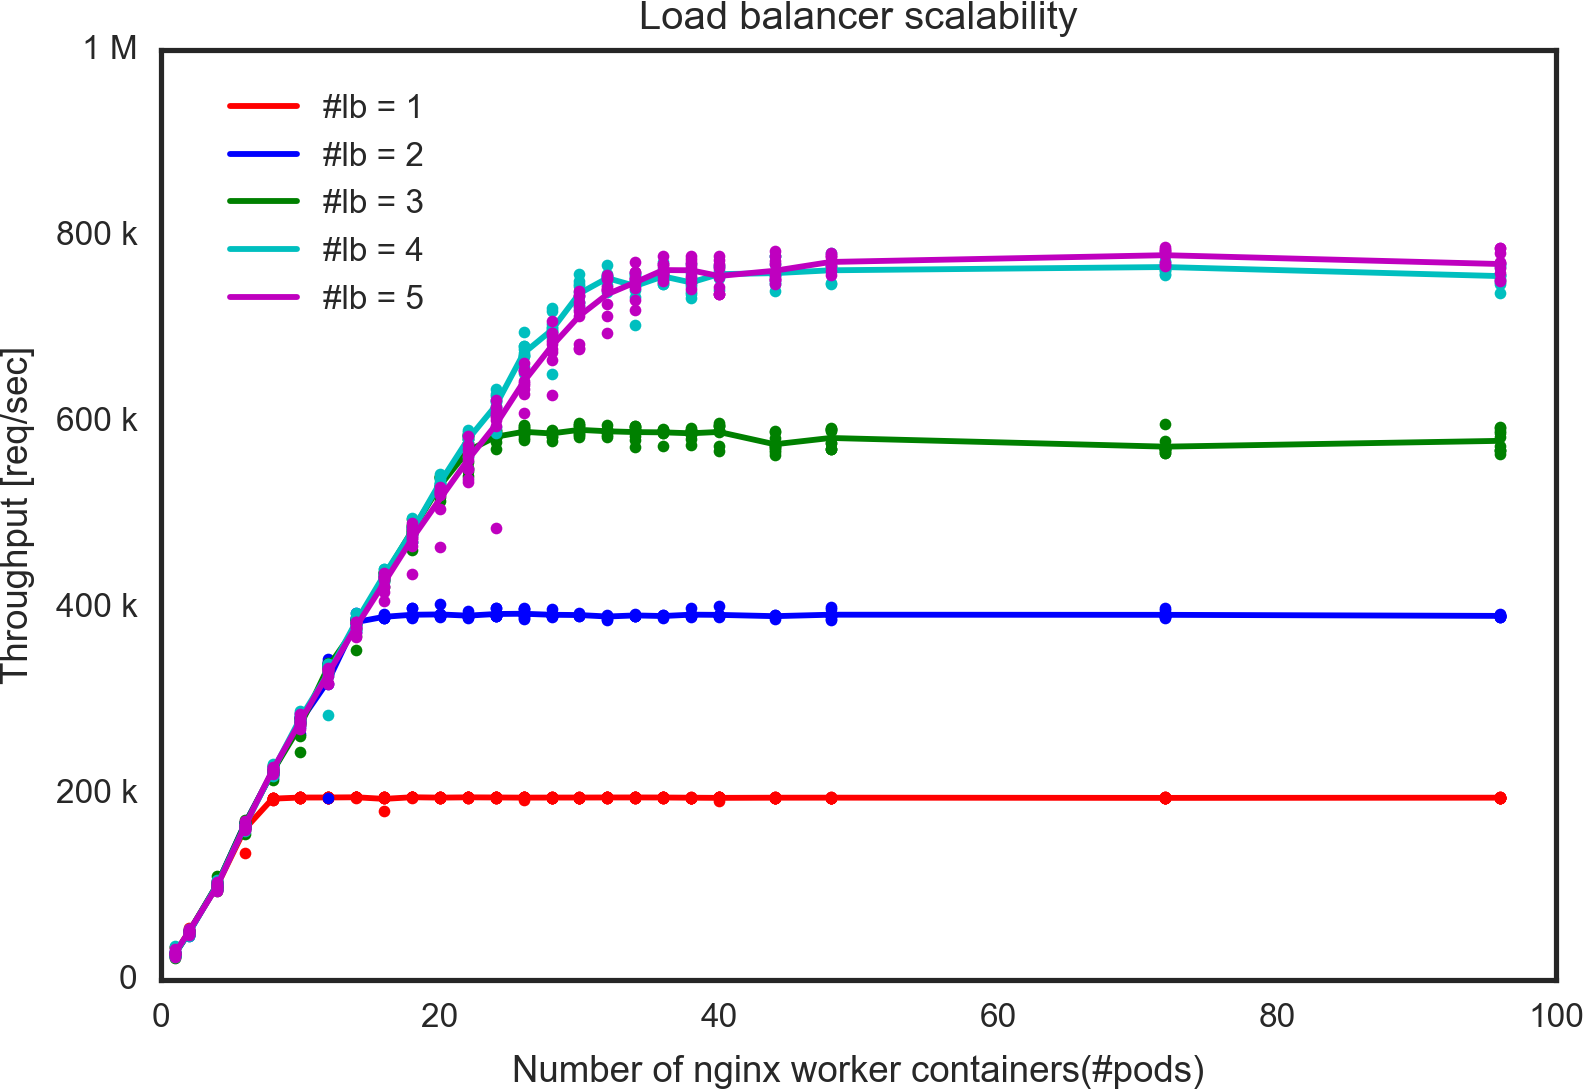
\includegraphics[width=0.9\columnwidth,left]{Figs/ecmp_lb_cubic}
  \caption{Caption 1}
  \label{fig:ecmp_lb_cubic}
\end{figure}

The throughput measurement was also carried out to show that ECMP technique increases the throughput as the number of the load balancers is increased.
Fig.~\ref{fig:ecmp_lb_cubic} shows the results of the measurements.
There are four solid lines in the figure, each corresponding the throughput result when there are one through four of the proposed load balancers.
As can be seen in the figure, as we increased the number of the pod the throughput increased linearly to a certain level after which it saturated.
The saturated levels, i.e. performance levels, depend on the number of the ipvs load balancer pods (lb x 1 being the case with one ipvs pods, and lb x2 being two of them and as such).
The performance levels increase linearly as we increase the number of the load balancers.

The performance level did not scale further when the number of load balancers was increased more than four.
This was because the performance of the benchmark client hit the ceiling, i.e., the CPU usage was 100\% when the total throughput was around 780k [req/sec].
The author expects that replacing the benchmark client with more powerful machines will improve the performance level further.

\FloatBarrier

\section{ECMP response}

\begin{figure}[t]
  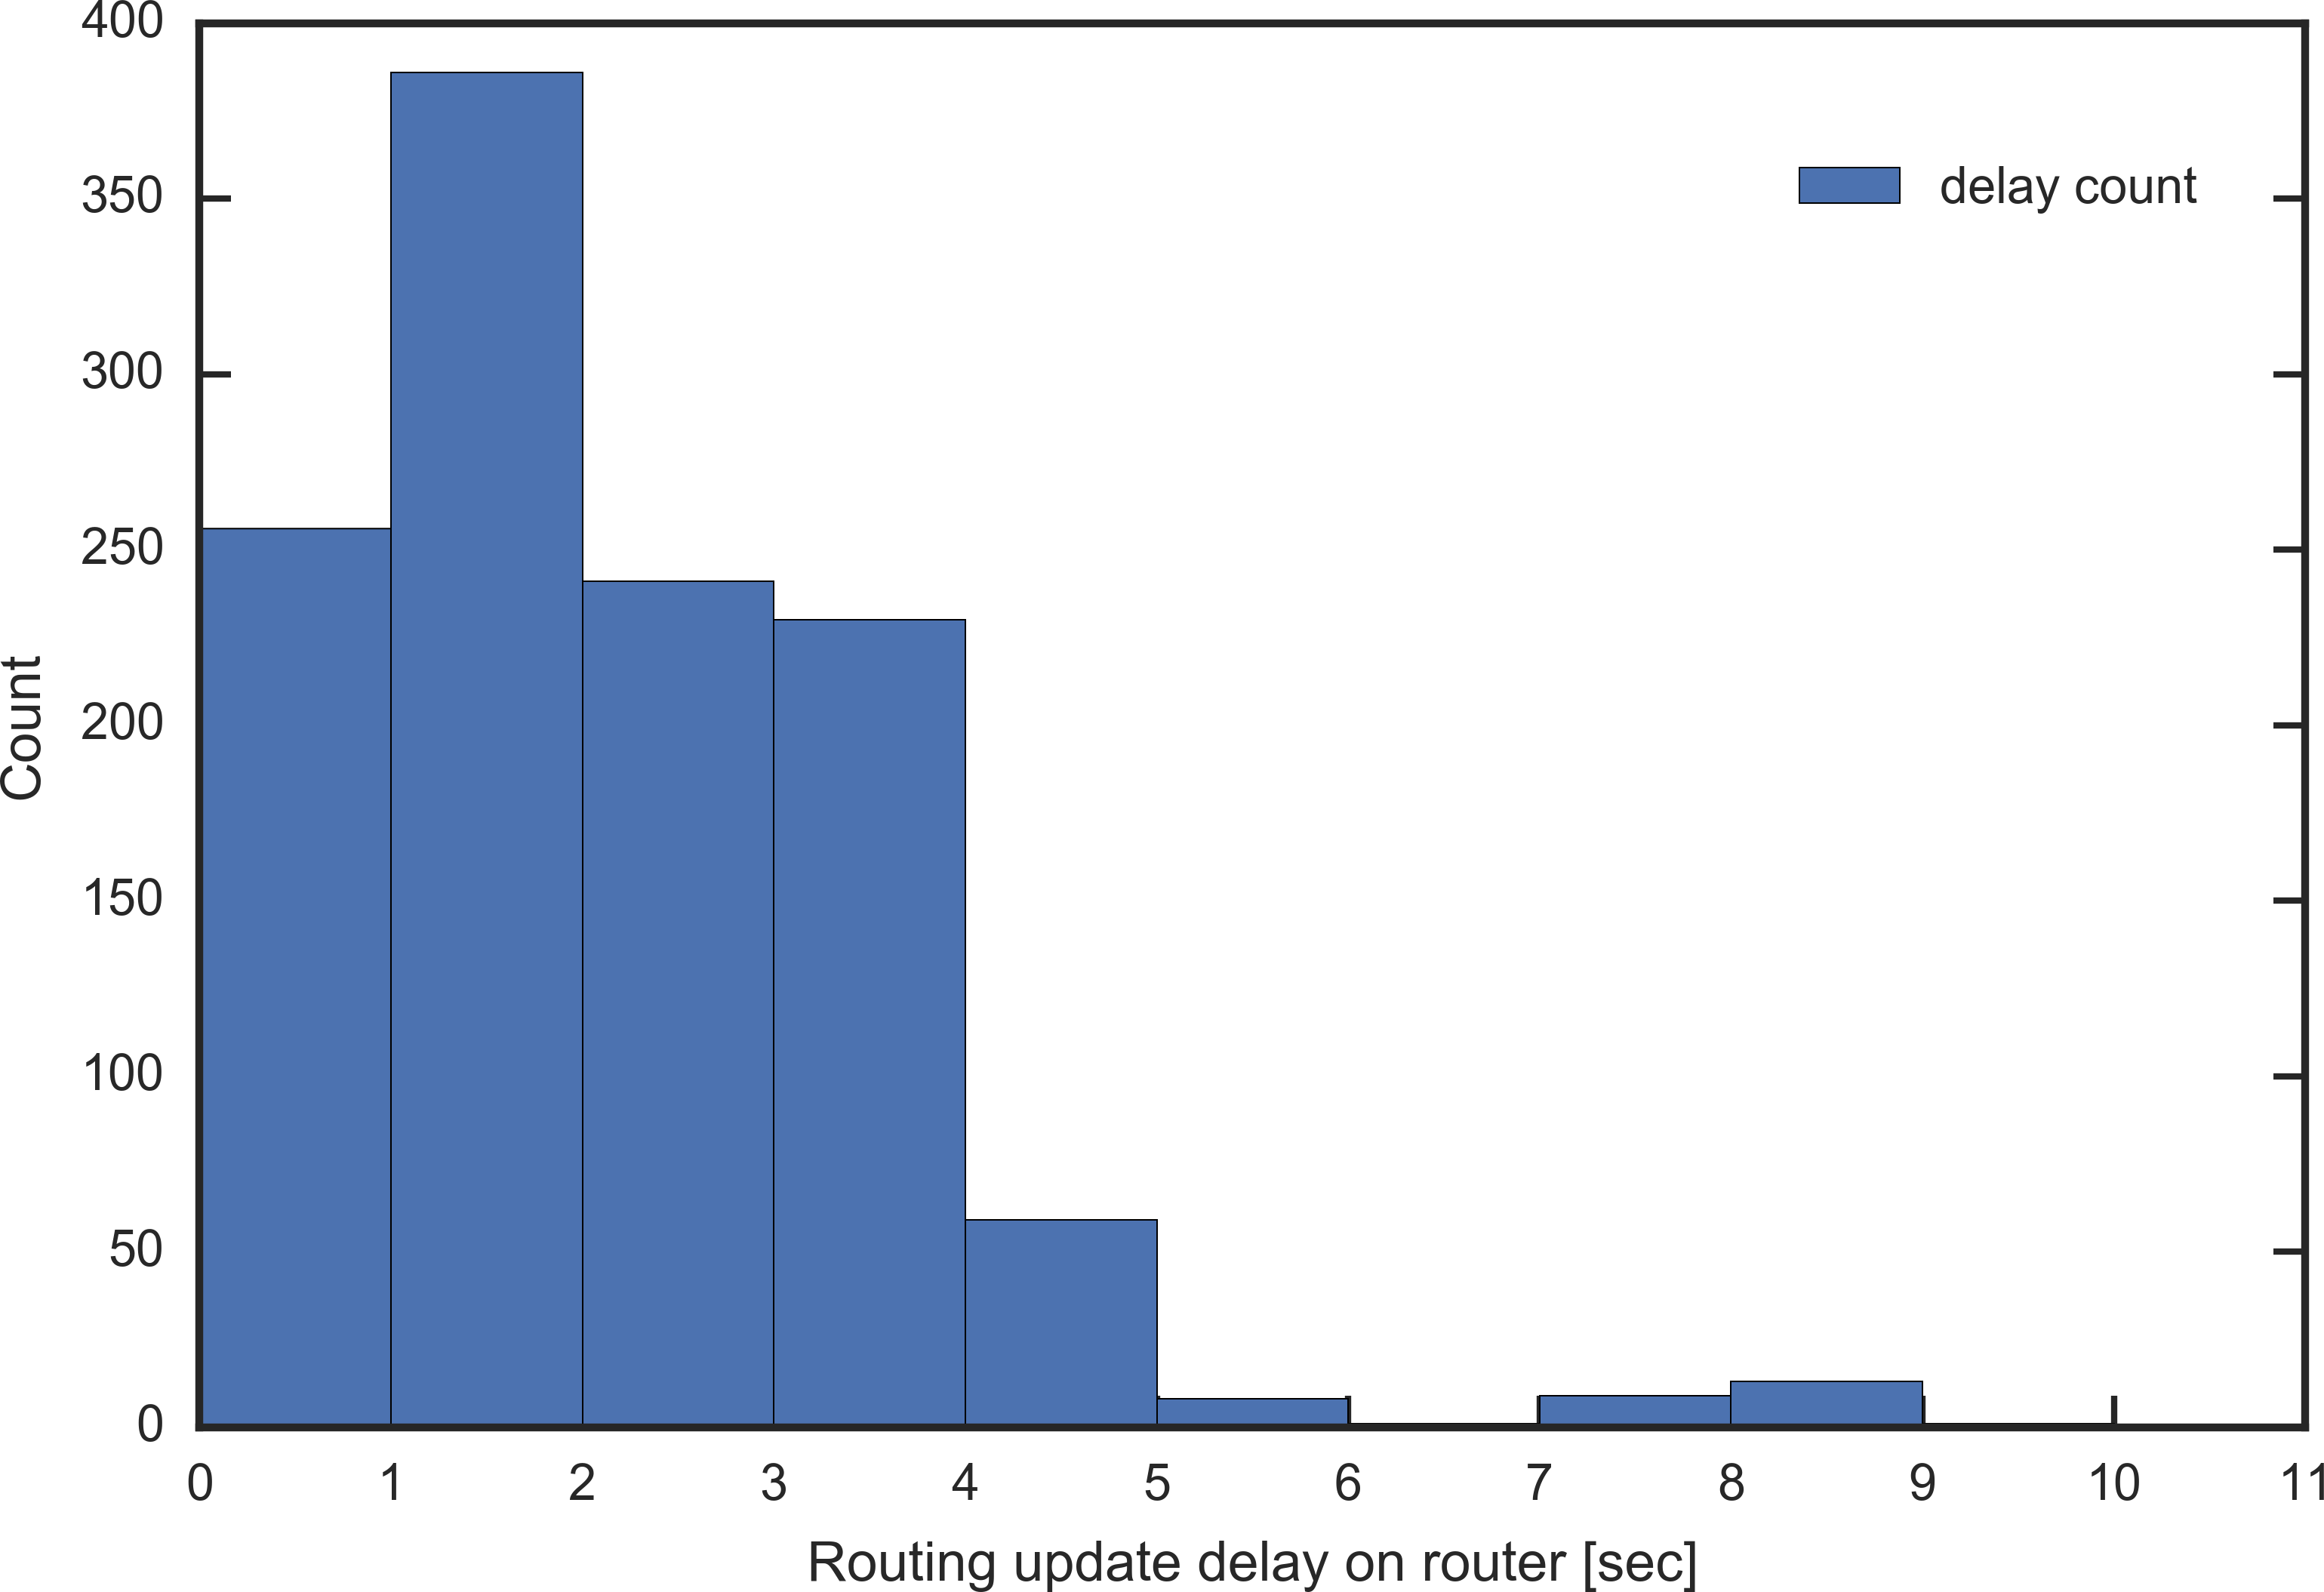
\includegraphics[width=0.9\columnwidth,left]{Figs/ecmp_delay_histgram}
  \caption{Caption 2}
  \label{fig:ecmp_delay_histgram}
\end{figure}

Figure~\ref{fig:ecmp_delay_histgram} shows the histogram of the ECMP update delay, where the author measured the delays until the number of running ipvs pods is reflected in the routing table on the benchmark client, as the number of the ipvs pods is changed randomly every 60 seconds for 20 hours.
As we can see from the figure, most of the delays are within 6 seconds, and the largest delay was 10 seconds.
We can conclude that ECMP routing update in our proposed architecture is quick enough.

\begin{figure}[t]
  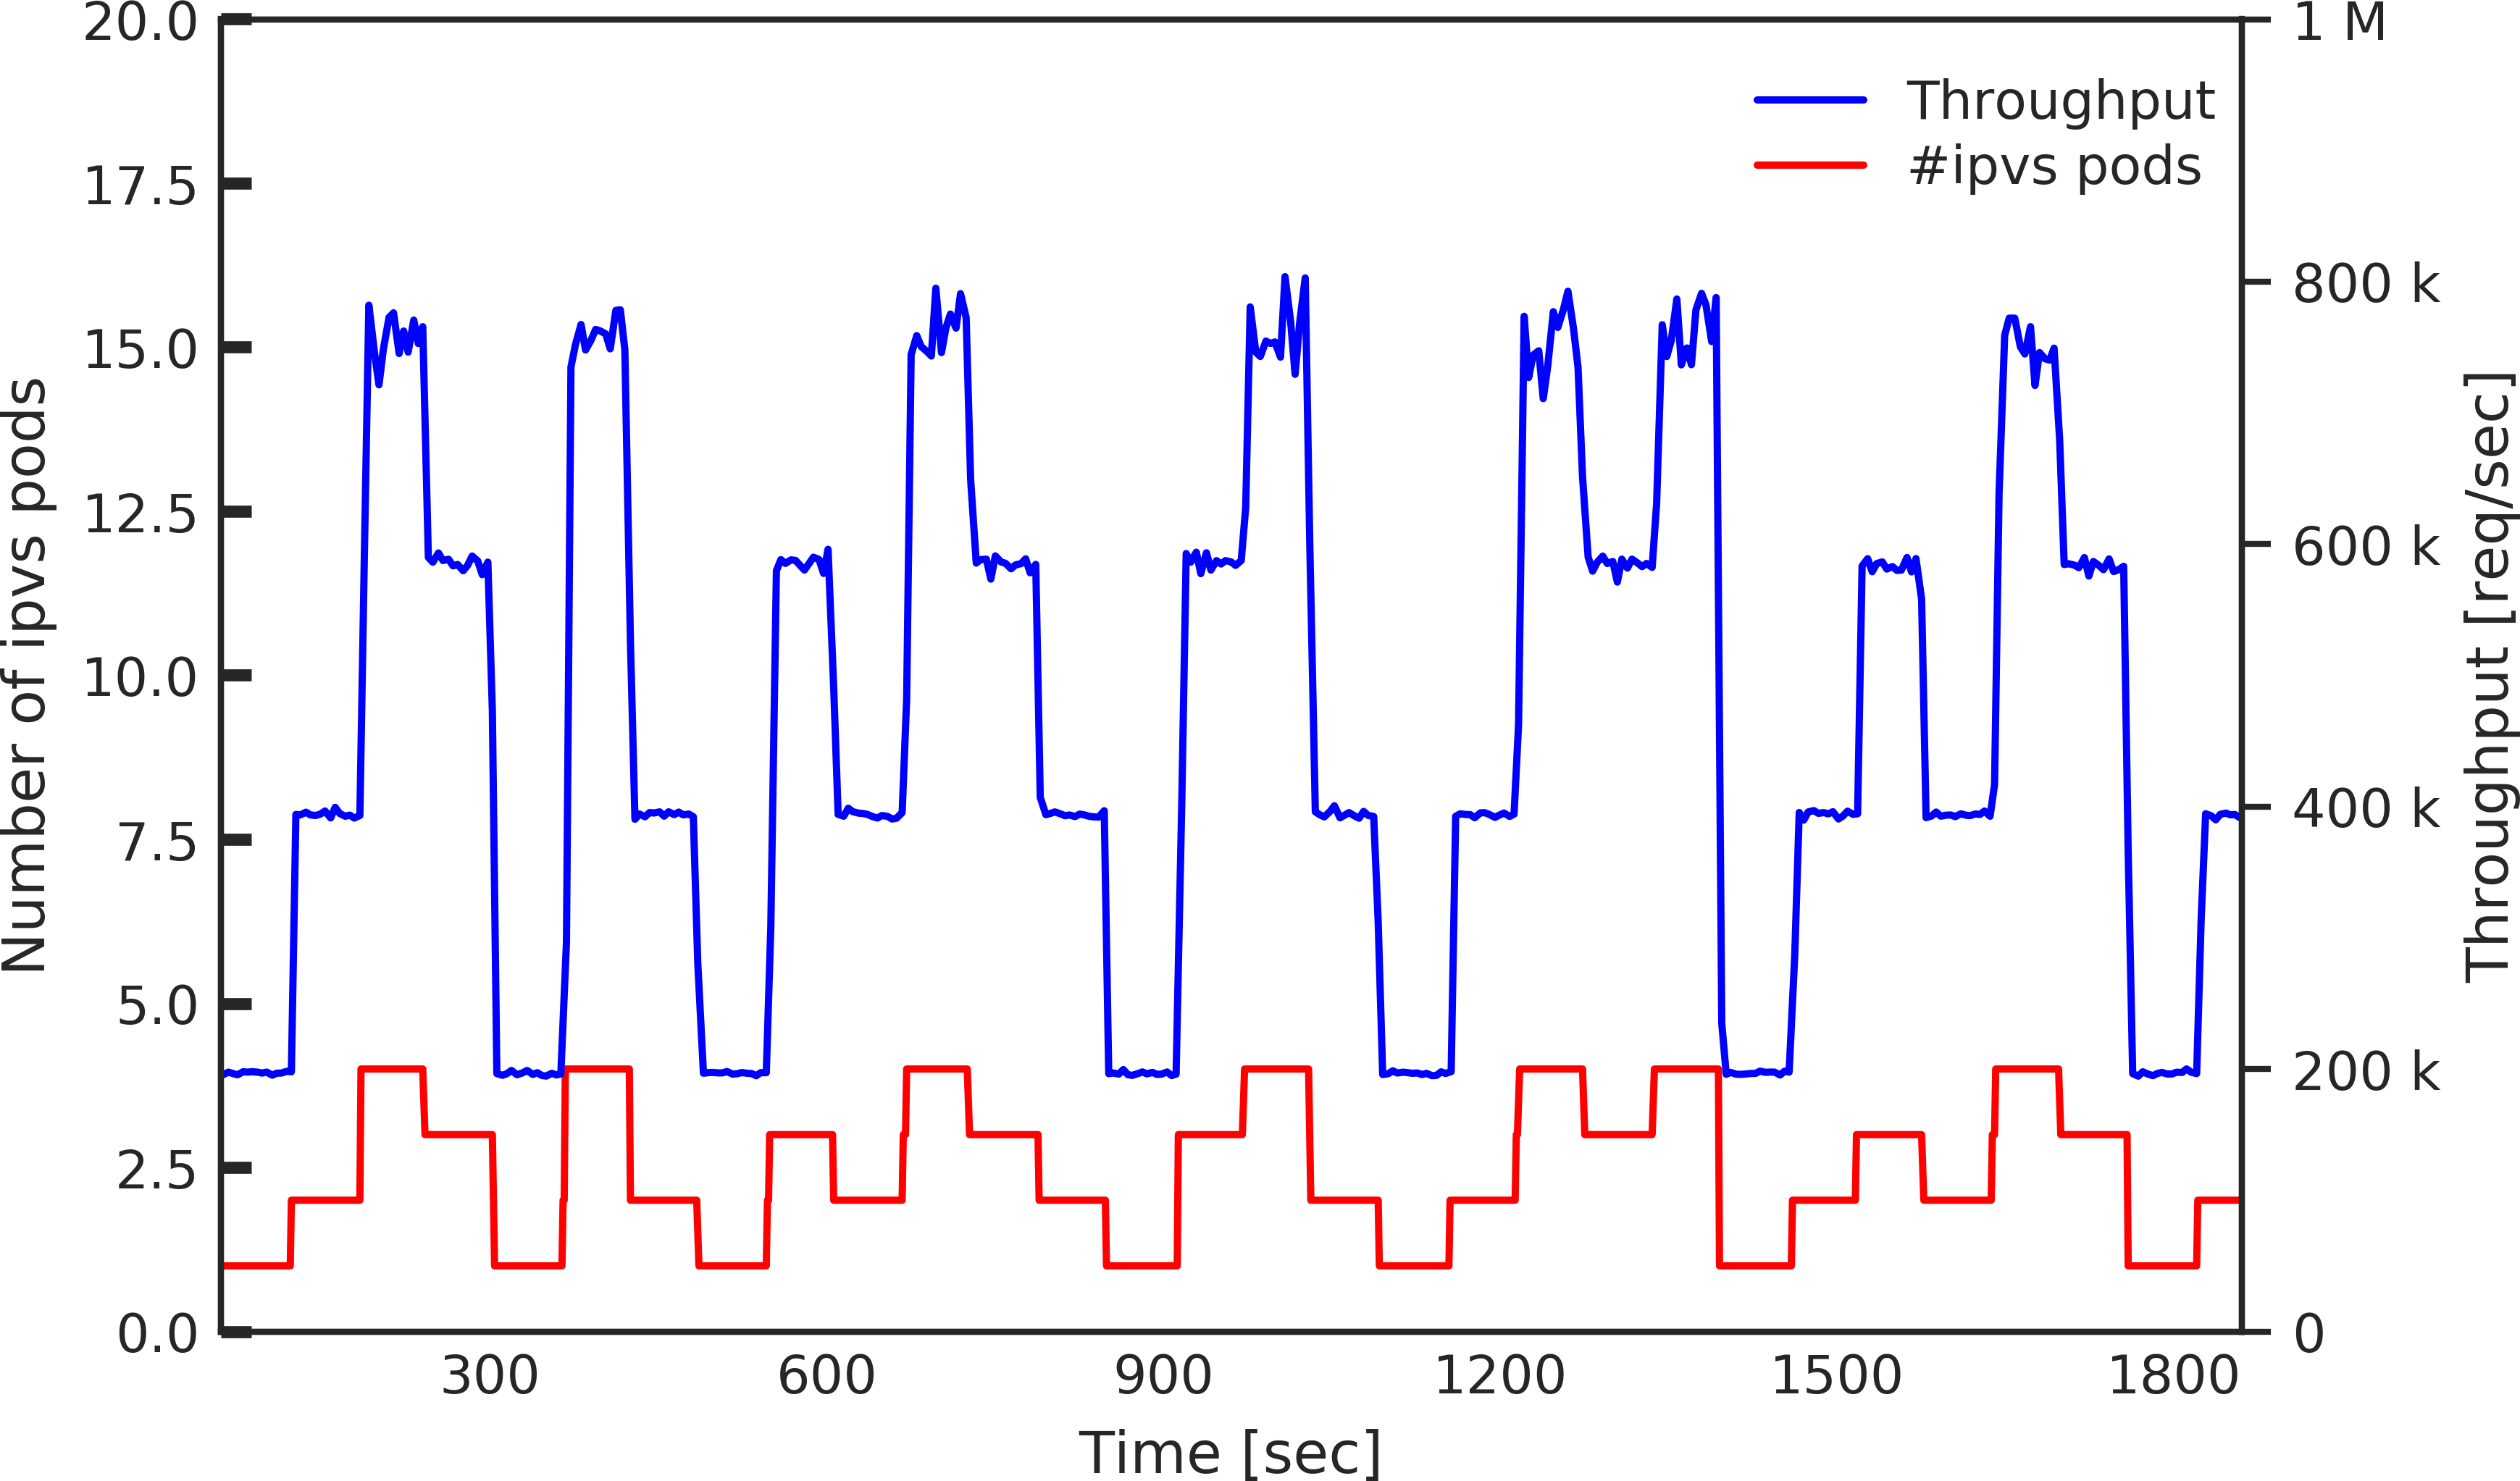
\includegraphics[width=0.98\columnwidth,left]{Figs/ecmp_response}
  \caption{Caption 2}
  \label{fig:ecmp_response}
\end{figure}

Figure~\ref{fig:ecmp_response} shows the throughput measurement results when the number of the load balancers was periodically changed. 
The red line in the figure shows the number of the ipvs load balancer pods, which was changed randomly every 60 seconds.
The blue line corresponds to the resulting throughput.
As we can see from the figure, the blue line nicely follows the shape of the red line.
This indicates that new load balancers are immediately utilized after they are created.
It also indicates that after removing some load balancers, the traffic to them is immediately directed to the existing load balancers.

\FloatBarrier

\section{Summary}

In this chapter, the redundancy and scalability of the proposed load balancers have been discussed.
The author verified that ECMP routing table was properly created in the experimental system.
The update of the ECMP routing table was correct and quick enough, i.e., within 10 seconds, throughout 20 hours experiment.
The scalability of the load balancer was also examined and it has been found that maximum performance levels scaled linearly as the number of the load balancer pods was increased to four.
The maximum throughput level obtained through the experiment was 780k [req/sec], which is limited due to the maximum CPU performance of the benchmark client rather than the performance of the load balancer cluster.


